\chapter{Data}\label{ch:data}

\begin{guide}
About 4--5 pages. Largely the proposal's ``Data and Preprocessing'' chapter, updated to what was actually done. Sources of truth: \texttt{Code/} (fetch and feature scripts), \texttt{DATA\_FREEZE.md}, \texttt{HANDOFF.md} (Phase 1).
\end{guide}

\section{Sources}
\tbc{table: series, source, frequency - BTC, ETH, S\&P 500, gold, dollar index, VIX, on-chain, volumes}

\section{Features}
\begin{guide}
List the 19 features that make up $X_t$ (a table works best): log-returns, realised volatility, rolling cross-asset correlations, on-chain and volume features. Give the formula for the log-return, $r_t = \ln(P_t / P_{t-1})$, once.
\end{guide}
\tbc{}

\section{Targets}
\begin{guide}
Three targets, stated precisely:
\begin{itemize}
  \item Alpha Agent: next-day BTC log-return $r_{t+1}$;
  \item Beta Agent volatility: the size of the next day's move, $|r_{t+1}|$ (changed from the proposal's 14-day rolling volatility - say so here and point to \cref{sec:vol-target});
  \item Beta Agent jump label: whether $|r_{t+1}|$ exceeds 3 rolling standard deviations \tbc{check exact definition in code}.
\end{itemize}
\end{guide}
\tbc{}

\section{Alignment, normalisation and splits}
\begin{guide}
Weekend/holiday alignment of stock-market series with 24/7 crypto; normalisation fitted on the training set only. Then the split, ideally with \texttt{explain\_btc\_splits.png} (a clean version of the BTC price with periods shaded).
\end{guide}

\begin{table}[ht]
  \centering
  \caption{Chronological data splits.}
  \label{tab:splits}
  \begin{tabular}{lll}
    \toprule
    Split & Period & Used for \\
    \midrule
    Training   & 2018 -- 2023 & fitting all models \\
    Validation & 2024 & early stopping, Platt scaling, Risk Engine tuning \\
    Test       & 2025 & reported results (touched once) \\
    Forward    & 1 Jan -- 30 Sep 2026 & untouched out-of-sample check (nothing retuned) \\
    \bottomrule
  \end{tabular}
\end{table}

\begin{figure}[ht]
  \centering
  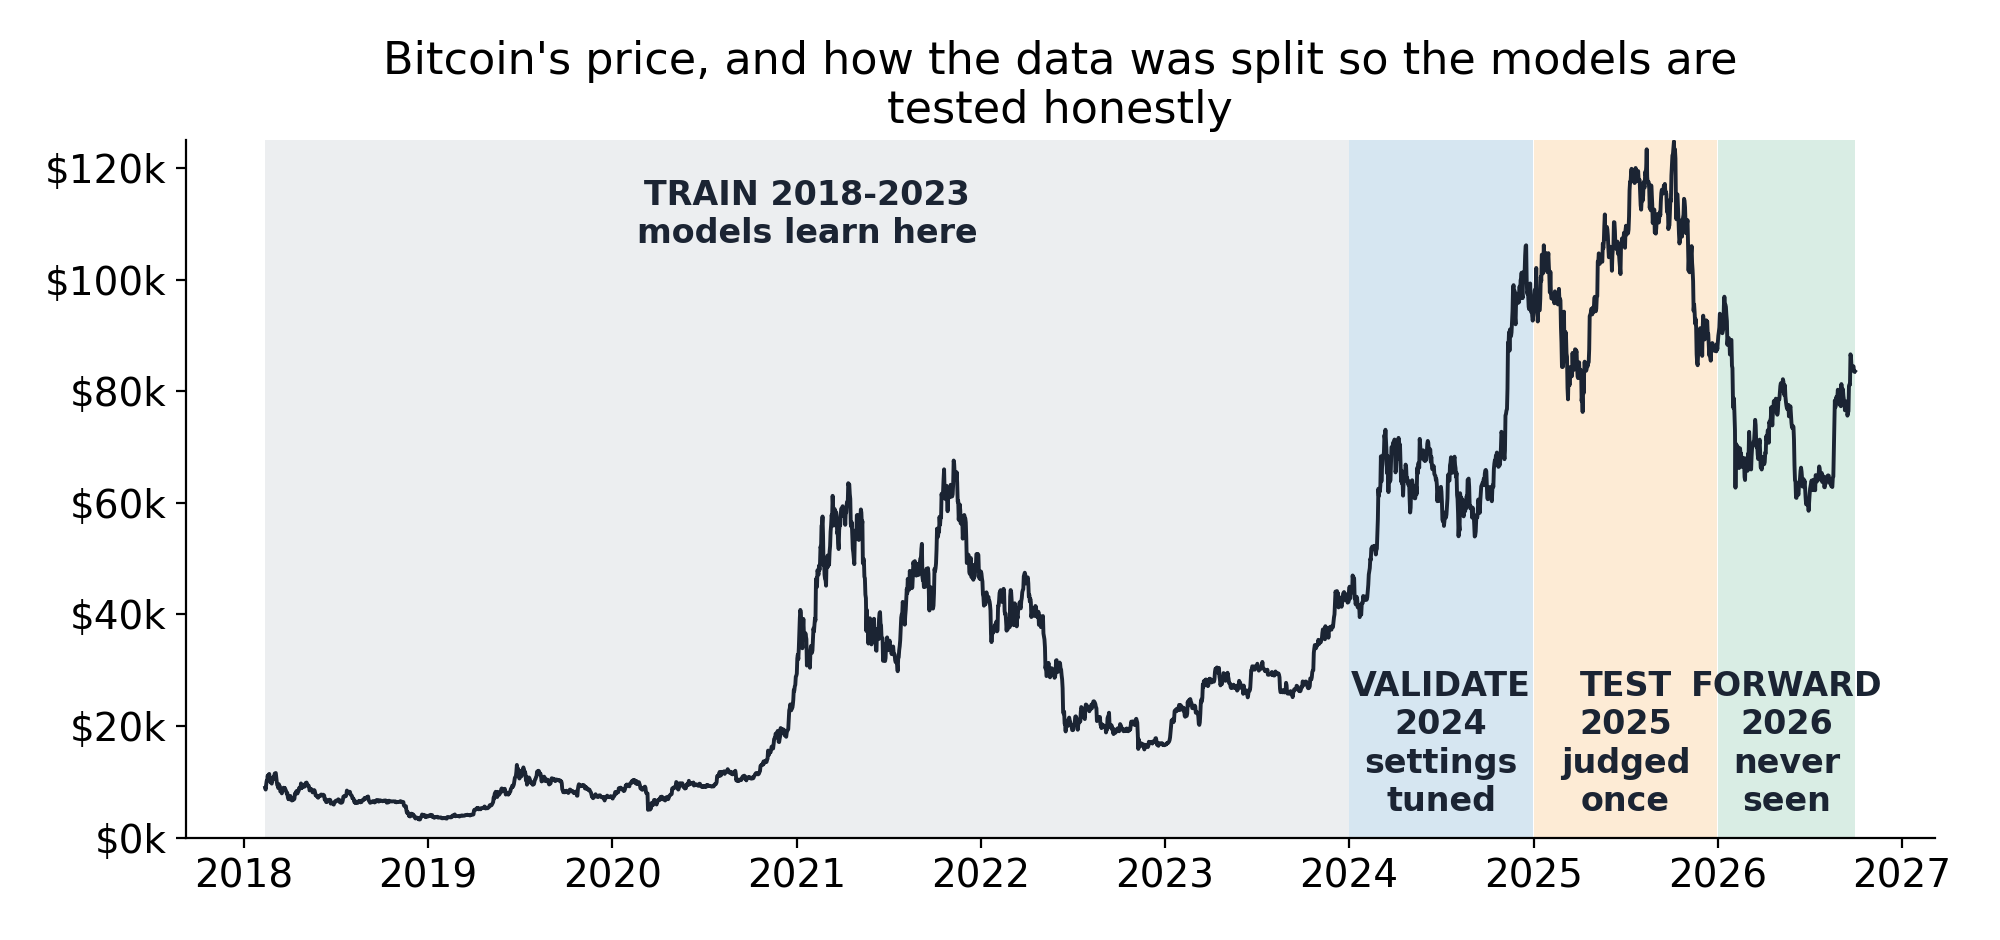
\includegraphics[width=0.85\textwidth]{explain_btc_splits.png}
  \caption{BTC price with the training, validation, test and forward periods. \tbc{redo caption}}
  \label{fig:splits}
\end{figure}

\section{Integrity checks}\label{sec:integrity}
\begin{guide}
This is a strength - spend a paragraph on it. A leakage audit (9 of 9 checks passed: no feature uses information from after day $t$), a mutation test (6 of 6: deliberately planted leaks were caught), and a data freeze with SHA-256 checksums (\texttt{DATA\_FREEZE.md}, git tag \texttt{data-freeze-2026-10-07}) so every number in this report can be reproduced. The 2026 forward data was fetched afterwards and checked against the frozen data (11 of 12 series identical over 2018--2025; gold differs by 0.10\% because of futures roll adjustments).
\end{guide}
\tbc{}
